\section{$k$-clique Problem}

$k$-clique Problem belongs to $\NPC$ problems, its task is to decide whether there exists a clique with $k$ vertices in given graph $G$ with $n$ vertices. Note that there exists a $k$-clique in $G$ iff there exists a $k$-independent set in $\overline{G}$ iff there exists an $(n-k)$-vertex cover of $\overline{G}$. Thus we can assume $k \leq \frac{n}{2}$ because those verification algorithms would be very similar.

From technical reasons we need $k$ to be even in all following examples; reduction from odd numbers will be solved in every single example.

Here if $k$ is odd, we add another vertex connected to every original vertex resulting in $G'$. Then existence of $(k+1)$-clique in $G'$ is equivalent to existence of $k$-clique in $G$. In following example in Figure \ref{fig:k-clique} we take $k$ even.

% reduction from SAT (wiki) ??

\subsection*{Set of tiles}

Here we describe tiles used by proposed DNA algorithm, Figure \ref{fig:k-clique} might be helpful. Moreover we give the leading term\footnote{See Definition \ref{def:O}. Note that in following text we will only give leading term(s).} of the amount of required tiles of given type in terms of $n$ -- number of vertices, $e$ -- number of edges and $k$ -- size of seeked clique.

\begin{description}
	\item[Bottom tiles.] There are tiles with non-colored $2l-2$ and $2l$ $(0 < l \leq \frac{k}{2})$ in this order on the bottom sides and with all possible numerically ordered\footnote{Later we will order by color.} combinations of numbers of connected vertices\footnote{Note that this restriction does not reduce the set of candidate $k$-cliques.} having $(k-2l+2)$-th and $(k-2l+1)$-th color, respectively, on the top sides. $e\cdot \frac{k}{2}$ tile types were required.
	\item[Bottom corner tiles.] Both bottom corner tiles are connected on the bottom by the lowest and the highest non-colored number, respectively, and have their special glue -- \# which can be viewed as $-\infty$ with respect to used ordering and * as $+\infty$, respectively -- on the top. $2$ tile types were required.
	\item[Inner tiles.] These tiles are responsible for ordering\footnote{Principially they are the same as in Winfree \cite{winfree_phd}.} by color during which they verify existence of every edge. There exist all 2-color combinations of all pairs of numbers of connected vertices in both number-orders with both correct and reverse color-order on the bottom and with correct color order of the same numbers on the top. Moreover there exist similar tiles with sharp and asterisk instead of left or right number, respectively, with an exception: sharp and lowest color, and asterisk and highest color do not exist, these are reserved for verification tiles. Remind that the top sharp or asterisk must have glue-strength $2$.
	
	As soon as there appear unconnected vertices' numbers next to each other, the self assembly cannot continue and reach ``DONE'' because no tile can connect to this place. Note that colors were generated in reverse color order so they must meet each other during color ordering. Every missing edge would be revealed thus ``DONE'' tile connects iff the generated subset is a clique. $2\cdot\binom{k}{2}\cdot 2e + 2(k-1)n \sim 2 k^2 e + 2kn$ tile types were required. %!% zkontrolovat, pro hranu se dělaj obě pořadí
	\item[Border tiles.] There are two tile types on the borders, one with sharps, one with asterisks. They just keep the structure growing up and signalize border. Remind that the bottom sharp or asterisk must have glue-strength $2$. $2$ tile types were required.
	\item[Verification tiles.] As soon as the lowest color reaches sharp and the highest color reaches asterisk there connect two special tiles which start verification whether nothing is missing. There exist two types of verification sequences ``C'' and ``D'' with all color--number combinations -- ``D'' with the smaller half (by color), ``C'' with the higher half. $kn$ tile types were required.
	\item[DONE tile.] If everything is verified and verification sequences meet each other, ``DONE'' tile will be connected to signalize correct solution. $1$ tile type was required.
\end{description}

Summed up, this DNA algorithm requires $2 k^2 e + 2 kn$ tile types. To compute Binding complexity easily we use following lemma.

\begin{lemma}
	In a square $\myatam$ tiling with $n$ bottom tiles there are $\sim 4 n^2$ bonds.
\end{lemma}
\begin{proof}
	Note that the square can be divided by diagonals into four triangles consisting of $\sim \frac{n^2}{2}$ tiles thus there are $\sim 2n^2$ tiles. Every inner tile has four bonds, every inner bond belongs to two tiles thus there are $\sim 4n^2$ bonds.
\end{proof}

Binding complexity is $1\nicefrac{1}{4} \cdot 4 \bigl(\frac{k}{2}\bigr)^2 = 1\nicefrac{1}{4}\,k^2$, glue complexity is $kn$.

\begin{figure}[H]
\begin{center}
	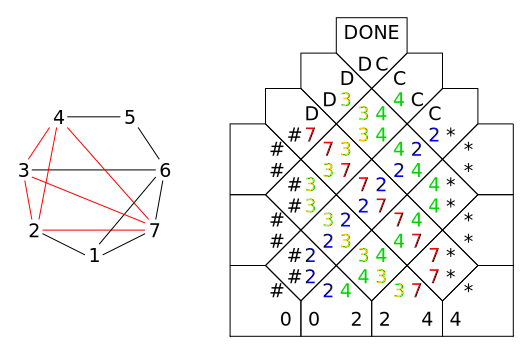
\includegraphics[scale=0.75]{./figures/k-clique/k-clique.pdf}
	\caption{$k$-clique computation. Color order is defined by their wavelength.}
	\label{fig:k-clique}
\end{center}
\end{figure}

